\section{分割方法}\label{sec:segmentation_method}

\subsection{背景介绍}

在下文中,我们将使用像素这一术语,即使它可以应用于体素。我们的算法可以在二维和三维中实现,只是改变了邻域(见\cref{fig:邻域})。由于我们处理的图像中,一个物体或区域具有像素值相似的特点,我们选择区域直方图的标准偏差 $\sigma$ 作为同质性标准。

\begin{figure}[htbp]
    \centering
    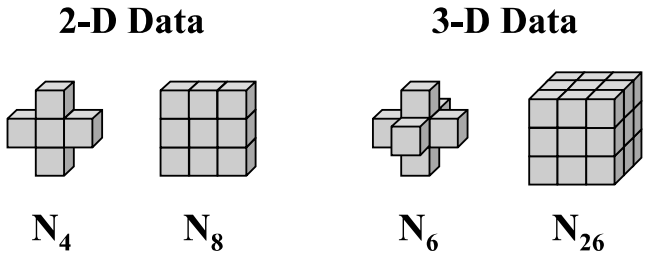
\includegraphics[width=0.5\textwidth]{figures/邻域.png}
    \caption{用于二维或三维实现的的邻域}
    \label{fig:邻域}
\end{figure}

\subsection{概述}

正如上一节所解释的,用区域生长技术分割的区域在很大程度上取决于最大同质性阈值σmax的选择。在交互式系统中,这个值是实验性地设置,并通过试验和错误来不断调整(Adams和Bischof,1994\cite{adams1994seeded})。在自动系统中,阈值的确定是比较麻烦的。它可以从初始种子的邻近像素进行评估。实际上,由于MR图像的局部不均匀性和弱信噪比(Antoniadis等人,1998\cite{antoniadis1998bone}),目标区域要么被分割得太多,要么被分割得太少。事实上,由于缺乏对要分割的区域的了解,在区域生长过程开始时确定最佳阈值是困难的。

在我们的方法中,分割的区域并不取决于 $\sigma_{max}$ 的初始值选择。\cref{fig:方法原理} 和 \cref{fig:流程图} 的流程图展示了对物体进行分割的步骤。在第一步中,一个含参区域增长算法使用一个给定区间内的每个 $\sigma_{max}$ 值对原始图像进行分割(见\cref{sec:初始化})。由此产生的按 $\sigma_{max}$ 升序排列的分割区域集合将被称为区域增长序列。与 $\sigma_{0}$($\sigma_{max}$ 的最小值)相对应的欠分割区域是该序列的第一个元素,与 $\sigma_{m}$($\sigma_{max}$ 的最大值)相对应的过分割区域是最后一个元素。在第二步中,对于序列中的每个元素,计算出一个代表分割质量评估的三维参数。这些取决于 $\sigma_{max}$ 的值被称为 $f_{a}(\sigma_{max})$ 评估函数(见 \cref{sec:assessment_function})。第三步是通过 $f_{a}(\sigma_{max})$ 确定序列中的最佳分割阈值 $\sigma_{opt}$ 。在本方法中,问题的解决被简化为一个最大函数检测。

\begin{figure}[htbp]
    \centering
    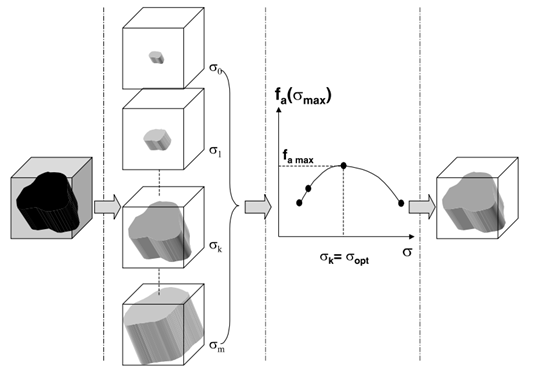
\includegraphics[width=0.7\textwidth]{figures/方法原理.png}
    \caption{方法原理}
    \label{fig:方法原理}
\end{figure}

\begin{figure}[htbp]
    \centering
    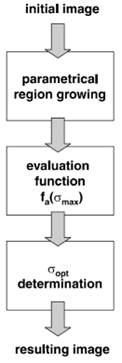
\includegraphics[width=0.2\textwidth]{figures/流程图.png}
    \caption{拟议方法的流程图}
    \label{fig:流程图}
\end{figure}

\subsection{ARG描述}\label{sec:arg_description}

\subsubsection{定义}
\begin{itemize}
    \item 一个区域 $R$ 被称为同质性,如果$\sigma \leq \sigma_{max}$,其中$\sigma_{max}$是一个给定的同质性阈值。
    \item 拉伸变换(Serra, 1982\cite{serra1982image}):考虑一个区域 $R$ 和一个邻域 $N$。根据定义,用 $N$ 对 $R$ 进行二元扩张得到的网格点集合 $D$ 是与 $R$ 相交的 $N$ 的平移中心的位置,这个集合用 $D=R \oplus N$ 表示。换言之:$D=\{x \in R |(N+x) \cap R \neq \emptyset\}$。
    \item 侵蚀变换(Serra, 1982\cite{serra1982image}):根据定义,用 $N$ 对 $R$ 进行二元侵蚀得到的网格点集合 $E$ 是包括在 $R$ 中的 $N$ 的平移中心的位置,这个集合用$E=R \ominus N$表示。换言之:$E=\{x \in R |(N+x) \subset R\}$。
    \item 收缩(Revol和Jourlin,1997\cite{revol1997new}):一个区域 $R$ 的 $k$ 收缩($k$-contraction)是通过移除所有属于 $R$ 的直方图的 $k$ 极端 非空隙的像素来获得的,$k$ 是直方图左边和右边的槽的数量。在本文中,我们使用这个定义的一个特殊情况,即所有被移除的像素都属于直方图的同一侧。我们称它为 $k$ 左收缩($k$-left-contraction)或 $k$ 右收缩($k$-right-contraction)。
    \item $RG(\sigma_{max}, \{S1,\dots,Sn\})$: 用 $\sigma_{max}$ 和 $\{S1,\dots,Sn\}$ 初始种子集得到的区域生长分割结果。为简单起见,下文将用 $R(\sigma_{max})$ 表示。
\end{itemize}

\subsubsection{种子和 $\sigma_{max}$ 范围的初始化}\label{sec:初始化}

当要分割的对象很紧凑时,区域生长可以只从一个种子开始。但当其形状比较复杂时,为了提高算法的速度,可能需要用许多种子开始区域生长。自动种子初始化有两个好处:(1)避免要求用户进行繁琐的工作;(2)确保分割结果的可重复性,因为种子的位置总是相同的。在我们的应用中,我们处理的是具有双峰柱状图的图像。种子的初始化可以通过粗略的分割来解决,如自动阈值化(Otsu, 1979\cite{otsu1979threshold}),然后再进行三维二元侵蚀(Serra, 1982\cite{serra1982image})。形态学操作确保了种子集被包括在要分割的对象中。尽管如此,在具有多模态直方图的图像的情况下,应该考虑另一种程序。

$\sigma_{max}$ 范围的初始化是由 $N_s$ 个初始种子 $S_i$ 和它们的相邻像素获得的(见\cref{fig:邻域})。对于每个种子 $S_i$ 和其相邻的像素,计算灰度等级的标准偏差 $\sigma_{S_i}$。设 $\sigma_{mean}$ 为 $\sigma_{S_i}$ 的平均值:
\begin{equation}
    \sigma_{mean}=\frac{\sum_{i = 0}^{N_s} \sigma_{S_i}}{N_s}
\end{equation}

其中 $\sigma_{mean}$ 为阈值范围的中间值,$\sigma_{0}$ 为范围的最小值,固定为 $(1-\beta) \sigma_{mean}$,$\sigma_{m}$ 为范围的最大值,为 $(1+\beta) \sigma_{mean}$。在我们的应用中,$\sigma_{max}$ 范围(即 $[\sigma_{0}, \sigma_{m}]$)将用 $\beta=0.5$ 时得到(即 $[0.5 \sigma_{mean}, 1.5 \sigma_{mean}]$)(见\cref{sec:test})。$\sigma_{max}$ 的步进 $\Delta \sigma$ 可以由用户固定,它将以 $\sigma_{mean}$ 的一个百分比给出。默认情况下,它将等于 $5\%$。

\subsubsection{区域生长过程}

区域增长过程的实现来源于以前的工作(Revol和Jourlin,1997\cite{revol1997new}),并因其能够分割非连接(non-connected)区域而被选中使用。在这种方法中,在某一步骤中属于同质区域 $R$ 的一些像素可以在后续步骤中被消除。这一特性限制了经典区域增长的连锁效应,并在需要分割的结构复杂时可以产生更好的区域增长分布。

根据我们的应用需要,该算法是针对具有双峰直方图的三维图像开发的。当需要分割的物体比背景更暗时,使用右收缩,否则使用左收缩:

在每一步,一个同质区域 $R_{n}$ 被一个邻域N扩张,产生一个区域 $D_{n+1}$,这个区域可能是同质的也可能不是。

如果区域 $D_{n+1}$ 是同质的(就 $\sigma_{max}$ 而言),$D_{n+1}$ 取代 $R_{n}$,我们前往下一步。

如果 $D_{n+1}$ 不是同质的,它就会被一个右缩或左缩的过程缩小,从而缩小其直方图的动态范围,产生一个同质的区域,称为 $C$,它取代了区域 $R_{n}$,然后我们前后下一步。

当区域 $R_{n}$ 不能再增加时,该算法就会停止。

区域增长过程的伪语言描述如下:

\begin{algorithm}
    \caption{区域增长过程}\label{algo:region_growing}
    \begin{algorithmic}[1]
        \State $n \gets 1$
        \State $R_{0} \gets \emptyset$
        \State $R_{1} \gets \{S_{1}, \ldots, S_{n}\}$
        \While{$R_{n} \neq R_{n-1}$}
            \State $D_{n+1} \gets R_{n} \oplus N$ \Comment{Dilation}
            \If{$\sigma_{D_{n+1}} \leq \sigma_{\max}$}
                \State $R_{n+1} \gets D_{n+1}$
                \State $n \gets n+1$
            \Else
                \State $k \gets 0$
                \While{$\sigma_{C} > \sigma_{\max}$}
                    \State $k \gets k+1$
                    \State $C \gets k \text{左收缩 of } D_{n+1} \text{ or } k \text{右收缩 of } D_{n+1}$
                \EndWhile
                \State $R_{n+1} \gets C$
                \State $n \gets n+1$
            \EndIf
        \EndWhile
        \State $\operatorname{RG}(\sigma_{\max},\{S_{1}, \ldots, S_{n}\}) \gets R_{n}$
    \end{algorithmic}
\end{algorithm}

\subsubsection{自动区域生长算法}

在第一次迭代中,$\{S_1,\dots,S_n\}$ 和 $\sigma_{max}$ 的范围如 \cref{sec:初始化} 所述被初始化。区域生长过程以 $\{S_1,\dots,S_n\}$ 和 $\sigma_{max}$(等于 $\sigma_0$) 对原始图像进行分割,得到一个分割区域 $RG(\sigma_{max},\{S_1,\dots,S_n\})$。在每一步,通过 $f_{a}(\sigma_{max})$ 评估所产生的分割,上述同质区域 $RG(\sigma_{max},\{S_1,\dots,S_n\})$ 取代 $\{S_1,\dots,S_n\}$,$\sigma_{max}$ 增加 $\Delta\sigma$,区域增长过程继续进行新的分割。当通过 $f_{a}(\sigma_{max})$ 确定与区域生长序列中的最佳分割相关的$\sigma_{opt}$时,该算法停止。该问题的解决相当于一个最大函数检测(见 \cref{sec:assessment_function})